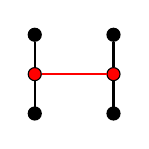
\begin{tikzpicture}[auto,scale=0.5]

	\node (c0) [circle, draw, fill=black, scale=0.5] at (0, 0) {};
	\node (c1) [circle, draw, fill=black, scale=0.5] at (0, 2) {};
	\node (c2) [circle, draw, fill=black, scale=0.5] at (2, 0) {};
	\node (c3) [circle, draw, fill=black, scale=0.5] at (2, 2) {};
	\node (c4) [circle, draw, fill=red, scale=0.5] at (0, 1) {};
	\node (c5) [circle, draw, fill=red, scale=0.5] at (2, 1) {};

	\path[thick]
	(c0) edge (c4)
	(c4) edge (c1)
	(c2) edge (c5)
	(c5) edge (c3)
	(c4) edge[red] (c5);

\end{tikzpicture}
